\Variant{19.02.2023}
\QQ{1}{Natural $a$ va $b$ sonlar uçun $a+b=111$ tenglik bajarilsa, $ab-1$ ayirmaning eng katta qiymatini toping.
\Opts{$2555$}{$3079$}{$110$}{$1$}}
\QQ{2}{Hisoblang:
\[\frac{1-3+5-7+9-11+\dots+2021-2023}{1-2+3-4+5-6+\dots+2021-2022}\]
\Opts{$\dfrac{1012}{1011}$}{$-1$}{$-1012$}{$1011$}}
\QQ{3}{Hisoblang:
\[\frac{10^{55}+10^{54}+10^{50}}{10^{49}+10^{53}+10^{54}}\]
\Opts{$100$}{$1$}{$10$}{$1000$}}
\QQ{4}{Ikki işçi bir işning $\dfrac23$ qismini $4$ kunda bajara oladi. Agar ular alohida işlasa, birinçi işçi işni ikkinçisidan $5$ kun oldinroq bajarib tugatadi. Yolğiz işlaganda birinçi işçi işni neça kunda tugata oladi?
\Opts{$10$}{$12$}{$15$}{$20$}}
\QQ{5}{$500$ kg rudadan temir miqdori $12{,}5\%$ bölgan $200$ kg ruda ajratib olindi. Natijada qolgan rudadagi temir uluşi dastlabkisidan $20$ foiz punktga ortiq böldi. Dastlab ruda tarkibida qança (kg) temir bölgan?
\Opts{$212{,}5$}{$202{,}5$}{$45$}{$205$}}
\QQ{6}{Hisoblang:
\[\sqrt{\frac{2022\cdot2024+1}{2024\cdot2030+9}\cdot\frac{2026\cdot2028+1}{2020\cdot2026+9}-1}+\sqrt{25}\]
\Opts{$2021$}{$2022$}{$6$}{$5$}}
\QQ{7}{Arifmetik progressiyada $a_5+a_{n-4}=24$ va $S_n=96$ bölsa, $n$ ni toping.
\Opts{$7$}{$9$}{$4$}{$8$}}
\QQ{8}{Birinçi hadi $5$ dan katta bölgan geometrik progressiyada $b_1+b_2+b_3=21$ va $b_3+b_4+b_5=84$ bölsa, uning dastlabki oltita hadining yiğindisini toping.
\Opts{$25$}{$-174$}{$20$}{$-147$}}
\QQ{9}{Ifodani soddalaştiring:
\[\frac{a^2+b^2}{a+b}:\left(\frac{a^2+b^2}{ab}+\frac{b^2}{a^2-ab}-\frac{a^2}{ab+b^2}\right)\]
\Opts{$1$}{$a^2+b^2$}{$a+b$}{$a-b$}}
\QQ{10}{Tenglamani yeçing:
\[x+\frac x{1+2}+\frac x{1+2+3}+\dots+\frac x{1+2+3+\dots+7}=7\]
\Opts{$5$}{$4$}{$3$}{$2$}}
\QQ{11}{Agar $a<a^3<a^2$, $b^3<b<b^2$, $c^3<c^2<c$ bölsa,
\[\frac{ab|b-c-1|}{|ab|}+\frac{bc|a+c+1|}{|bc|}+\frac{ac|a+1+b|}{|ac|}\]
ifodani soddalaştiring.
\Opts{$1$}{$-1$}{$-2a-2b-2c-3$}{$a+b$}}
\QQ{12}{Soddalaştiring:
\[2\tg53^\circ\left(\frac1{\sin106^\circ}+\frac1{\tg106^\circ}\right)\]
\Opts{$\tg^253^\circ$}{$1$}{$2$}{$\tg53^\circ$}}
\QQ{13}{Agar $a-b=4$ bölsa, $\dfrac{a^2-b^2+3a-3b}{a^2-b^2+6a+9}$ ni hisoblang.
\Opts{$\dfrac14$}{$\dfrac74$}{$1$}{$\dfrac47$}}
\QQ{14}{$2^x+3^x+4^x+5^x>54$ tengsizlikning $[2;\,2023]$ oraliğida neçta natural yeçimi bor?
\Opts{$2021$}{$2023$}{$0$}{$2022$}}
\QQ{15}{Quyidagi funksiyalardan neçtasi toq?
\[1)\ y=2^x+2^{-x}\qquad 2)\ y=x\sqrt{1+x^2}\qquad 3)\ y=1+\sin2x\qquad 4)\ y=\log_2\left(x+\sqrt{1+x^2}\right)\]
\Opts{$1$}{$2$}{$3$}{$4$}}
\QQ{16}{Tenglamaning haqiqiy ildizlari sonini toping.
\[x^2+\frac{4x^2}{(5x+2)^2}=\frac95\]
\Opts{$4$}{$3$}{$2$}{$1$}}
\QQ{17}{$|x+y-12|+(x-y-2)^2=0$ tenglamani qanoatlantiruvçi $x$ va $y$ uçun $x\cdot y$ ni hisoblang.
\Opts{$25$}{$28$}{$30$}{$35$}}
\QQ{18}{Tengsizlik $[1;\,2023]$ kesmada neçta natural yeçimga ega?
\[\frac{\pi x-\sqrt{10}}{\pi-\sqrt{10}}<0\]
\Opts{$2023$}{$2021$}{$1$}{$2022$}}
\QQ{19}{Agar aholining elektr energiyasiga talabi har yili $2{,}5\%$ ortsa, neça yilda $9$ marta ortadi?
\Opts{$\log_91{,}025$}{$\log_90{,}025$}{$\log_{1{,}025}9$}{$\log_{0{,}025}9$}}
\QQ{20}{Tengsizlikning butun yeçimlari neçta?
\[3^{\log_3\sqrt{5-x}}>3^{\log_3(x-4)}\]
\Opts{$3$}{$2$}{$4$}{$0$}}
\QQ{21}{Tengsizlikning $[-4;\,5]$ oraliğidagi butun yeçimlari yiğindisini toping.
\[(2x+3)\left(x^2+3x\right)-\frac{16(2x+3)}{x^2+3x}\ge0\]
\Opts{$15$}{$9$}{$8$}{$10$}}
\QQ{22}{$y=\cos^nx\cdot\cos nx$ bölsa, $y'(x)$ ni toping.
\Opts{$n\cos^{n-1}x\cdot\sin(nx-x)$}{$-n\cos^{n-1}x\cdot\cos(nx+x)$}{$-n\cos^{n-1}x\cdot\sin(nx+x)$}{$n\cos^{n-1}x\cdot\sin(nx+x)$}}
\QQ{23}{Soddalaştiring:
\[\frac1{\cos x\cos2x}+\frac1{\cos2x\cos3x}+\frac1{\cos3x\cos4x}+\dots+\frac1{\cos2022x\cos2023x}\]
\Opts{$\dfrac{\sin2022x}{\sin2x\cos2023x}$}{$\dfrac{\sin2023x}{\cos x\cos2022x}$}{$\dfrac{2\sin2022x}{\sin2x\cos2023x}$}{$\dfrac{2\sin2022x}{\cos x\cos2023x}$}}
\QQ{24}{Aylanada $A$, $B$, $C$, $D$ nuqtalar olingan. $O$ — aylana markazi, $A$ va $D$ nuqtalar bilan bir töğri çiziqda yotadi. Agar $\angle ABC=30^\circ$ va $OD=3$ bölsa, $CD$ ni toping.
\qfig{\begin{tikzpicture}[scale=0.55,font=\small]
\coordinate (O) at (0,0); \coordinate (A) at (165:3); \coordinate (B) at (70:3); \coordinate (C) at (225:3); \coordinate (D) at (-15:3);
\draw (O) circle (3); \draw (A)--(B)--(C); \draw (O)--(D); \fill (O) circle (2pt);
\node at ($(B)+(-0.45,-0.75)$) {\scriptsize$30^\circ$};
\node[left] at (A) {$A$}; \node[above right] at (B) {$B$}; \node[below left] at (C) {$C$}; \node[right] at (D) {$D$}; \node[below left] at (O) {$O$};
\end{tikzpicture}}
\Opts{$3$}{$4$}{$\sqrt3$}{$3\sqrt3$}}
\QQ{25}{$ABC$ uçburçakda $AD$, $BN$, $CM$ medianalar kesişgan nuqta $G$ bölsin. Agar $ABC$ uçburçak yuzasi $48$ ga teng bölsa, $GDN$ uçburçak yuzasini toping.
\qfig{\begin{tikzpicture}[scale=0.62,font=\small]
\coordinate (A) at (0,0); \coordinate (C) at (6,0); \coordinate (B) at (3.8,3.4); \coordinate (D) at ($(B)!0.5!(C)$); \coordinate (N) at ($(A)!0.5!(C)$); \coordinate (M) at ($(A)!0.5!(B)$); \coordinate (G) at ($1/3*(A)+1/3*(B)+1/3*(C)$);
\fill[qfill] (G)--(D)--(N)--cycle;
\draw (A)--(B)--(C)--cycle; \draw (A)--(D); \draw (B)--(N); \draw (C)--(M); \draw (G)--(D)--(N)--cycle;
\node[below left] at (A) {$A$}; \node[above] at (B) {$B$}; \node[below right] at (C) {$C$}; \node[right] at (D) {$D$}; \node[below] at (N) {$N$}; \node[above left] at (M) {$M$}; \node[above left] at (G) {$G$};
\end{tikzpicture}}
\Opts{$5$}{$4$}{$3$}{$12$}}
\QQ{26}{$A(-10;\,-3)$, $B(-4;\,5)$, $C(5;\,5)$, $D(11;\,-3)$ nuqtalardan ötuvçi aylana radiusini toping.
\Opts{$10\dfrac58$}{$11\dfrac58$}{$8\dfrac34$}{$7\dfrac34$}}
\QQ{27}{Tomoni $4$ bölgan muntazam oltiburçak uçta tomonining örtalarini tutaştirib muntazam uçburçak yasalgan. Böyalgan soha yuzini toping.
\qfig{\begin{tikzpicture}[scale=0.42,font=\small]
\coordinate (L) at (-4,0); \coordinate (R) at (4,0); \coordinate (T1) at (-2,3.464); \coordinate (T2) at (2,3.464); \coordinate (B1) at (-2,-3.464); \coordinate (B2) at (2,-3.464);
\coordinate (M) at (0,3.464); \coordinate (P) at (-3,-1.732); \coordinate (Q) at (3,-1.732);
\coordinate (X1) at (-1,1.732); \coordinate (Y1) at (0.5,2.598); \coordinate (X2) at (1,-1.732); \coordinate (Y2) at (2.5,-0.866);
\fill[qfill] (P)--(X1)--(Y1)--cycle; \fill[qfill] (P)--(X2)--(Y2)--cycle;
\draw (L)--(T1)--(T2)--(R)--(B2)--(B1)--cycle; \draw (M)--(P)--(Q)--cycle; \draw (L)--(T2); \draw (B1)--(R); \draw (P)--(Y1); \draw (P)--(Y2);
\end{tikzpicture}}
\Opts{$1$}{$6\sqrt3$}{$2\sqrt3$}{$\sqrt3$}}
\QQ{28}{Tekis burçagi $60^\circ$ bölgan ikki yoqli burçakning qirrasida $A_1$ va $B_1$ nuqtalar olingan. Ulardan ikki yoqli burçakning turli yoqlarida $A$, $B$ nuqtalar burçakning qirrasiga perpendikulyar qilib $AA_1=16$ va $BB_1=13$. Agar $A_1B_1=17$ bölsa, $AB$ ni toping.
\qfig{\begin{tikzpicture}[scale=0.65,font=\small]
\fill[qfill!45] (-1.3,2)--(0,0)--(6.6,-0.3)--(5.3,1.7)--cycle; \fill[qfill!20] (0,0)--(6.6,-0.3)--(5.6,-2.1)--(-1,-1.8)--cycle;
\draw (-1.3,2)--(0,0)--(6.6,-0.3)--(5.3,1.7)--cycle; \draw (0,0)--(-1,-1.8)--(5.6,-2.1)--(6.6,-0.3);
\coordinate (A1) at (1.4,-0.064); \coordinate (A) at (1.4,1.3); \coordinate (B1) at (4.7,-0.214); \coordinate (B) at (4.7,-1.5);
\draw (A)--(A1); \draw (B)--(B1); \draw (A)--(B);
\draw (A1)++(0,0.2)--++(0.2,0)--++(0,-0.2); \draw (B1)++(0,-0.2)--++(-0.2,0)--++(0,0.2);
\draw (-0.35,0.55) arc (120:240:0.6); \node[left] at (-0.6,0) {$60^\circ$};
\node[above] at (A) {$A$}; \node[below] at (A1) {$A_1$}; \node[above] at (B1) {$B_1$}; \node[right] at (B) {$B$};
\node[left] at (1.4,0.65) {$16$}; \node[right] at (4.7,-0.85) {$13$}; \node[above] at (3.05,-0.14) {$17$};
\end{tikzpicture}}
\Opts{$\sqrt{202}$}{$\sqrt{53}$}{$6\sqrt2$}{$\sqrt{506}$}}
\QQ{29}{$y=ax^2+bx+c$ funksiya uçun $f'(1)=0$, $f(2)-f'(2)=1$ va $\displaystyle\int_0^1f(x)\,dx=\frac23$ bölsa, $b-a-c$ ni toping.
\Opts{$\dfrac14$}{$\dfrac34$}{$1$}{$0$}}
\QQ{30}{$ABCDA_1B_1C_1D_1$ kubda $\overrightarrow{BC}+\overrightarrow{CD}$ va $\overrightarrow{D_1A_1}+\overrightarrow{A_1B}$ vektorlar orasidagi burçak kosinusini toping.
\qfig{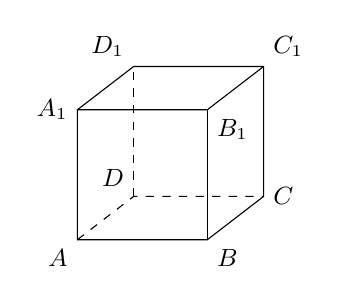
\begin{tikzpicture}[scale=0.55,font=\small]
\coordinate (A) at (0,0); \coordinate (B) at (3,0); \coordinate (C) at (4.3,1); \coordinate (D) at (1.3,1);
\coordinate (A1) at (0,3); \coordinate (B1) at (3,3); \coordinate (C1) at (4.3,4); \coordinate (D1) at (1.3,4);
\draw (A)--(B)--(C)--(C1)--(D1)--(A1)--cycle; \draw (A1)--(B1)--(C1); \draw (B)--(B1); \draw[dashed] (A)--(D)--(C); \draw[dashed] (D)--(D1);
\node[below left] at (A) {$A$}; \node[below right] at (B) {$B$}; \node[right] at (C) {$C$}; \node[above left] at (D) {$D$};
\node[left] at (A1) {$A_1$}; \node[below right] at (B1) {$B_1$}; \node[above right] at (C1) {$C_1$}; \node[above left] at (D1) {$D_1$};
\end{tikzpicture}}
\Opts{$\dfrac{\sqrt6}3$}{$\dfrac{\sqrt3}2$}{$\dfrac{\sqrt3}4$}{$-\dfrac{\sqrt6}3$}}
\QQ{31}{$A$ töplamning elementlari soni $9$ ta, $B$ töplamning elementlari soni $7$ ta, $U$ universal töplam elementlari soni $16$. $n(A\cup B)'$ eng köpi bilan neçaga teng? ($A'$ — $A$ töplamning universal töplamgaça töldiruvçisi.)
\Opts{$7$}{$13$}{$17$}{$11$}}
\QQ{32}{$10$ kişidan $1$ ta boşliq, $2$ ta yordamçi, $2$ ta mutaxassisni neça xil usulda tanlaş mumkin?
\Opts{$7850$}{$7560$}{$3780$}{$3840$}}
\QQ{33}{\Moslash{Gipotenuzasi $4\sqrt2$ bölgan töğri burçakli uçburçakning töğri burçagi uçidagi bissektrisasi uni ikkita teng yonli uçburçakka ajratadi. Berilgan uçburçak gipotenuza atrofida $360^\circ$ ga aylantirildi. ($\pi\approx3$ deb oling.)}{A) $16\sqrt2$\par B) $32$\par C) $32\sqrt2$\par D) $48\sqrt2$\par E) $30\sqrt2$\par F) $15\sqrt2$}{Hosil bölgan jismning töla sirtini toping.}{Hosil bölgan jismning hajmini toping.}{Hosil bölgan jismga içki çizilgan şar hajmini toping.}}
\QQ{36}{Tenglama berilgan:
\[\left(x^2-x-1\right)^3+\left(x^2-3x+2\right)^3=\left(2x^2-4x+1\right)^3\]
\AB{Tenglamaning neçta haqiqiy ildizi bor?}{Tenglamaning neçta musbat ildizi bor?}}
\QQ{37}{Tenglama berilgan:
\[\frac{\sin2^x}{\sin2^{x-2}\cos2^{x-2}}=2\sqrt3\]
\AB{Tenglamaning $(0;\,5)$ oraliqda neçta ildizi bor?}{Tenglamaning $(0;\,5)$ oraliqdagi eng katta va eng kiçik ildizlari ayirmasini toping.}}
\QQ{38}{$y=g'(x)$ funksiya grafigi parabola bölib, $(2;\,7)$, $(4;\,3)$, $(6;\,-9)$ nuqtalardan ötişi maʼlum.
\qfig{\begin{tikzpicture}[x=0.55cm,y=0.17cm,font=\small]
\draw[-{Stealth[length=4pt]}] (-2,0)--(8,0) node[right] {$x$}; \draw[-{Stealth[length=4pt]}] (0,-12)--(0,10) node[left] {$y$};
\draw[thick,domain=-1:6.4,samples=60] plot (\x,{-\x*\x+4*\x+3});
\foreach \p in {(2,7),(4,3),(6,-9)} \fill \p circle (2.5pt);
\node[above] at (2,7) {$(2;7)$}; \node[right] at (4,3) {$(4;3)$}; \node[right] at (6,-9) {$(6;-9)$}; \node[left] at (-1,-3) {$g'(x)$};
\end{tikzpicture}}
\AB{$y=g(x)$ funksiya grafigiga $x_0=-2$ nuqtada ötkazilgan urinmaning burçak koeffitsiyentini toping.}{$y=g(x)$ funksiyaning statsionar nuqtalari yiğindisini toping.}}
\QQ{39}{$ABCD$ kvadrat $BD$ diagonalining $D$ uçi davomida $E$ nuqta olingan va $DE=3$.
\qfig{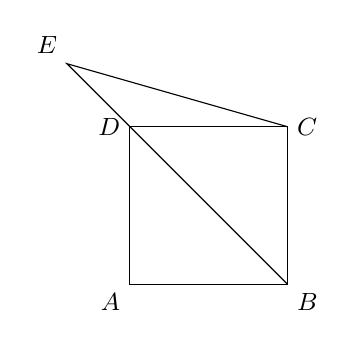
\begin{tikzpicture}[scale=0.5,font=\small]
\coordinate (A) at (0,0); \coordinate (B) at (4,0); \coordinate (C) at (4,4); \coordinate (D) at (0,4); \coordinate (E) at (-1.6,5.6);
\draw (A)--(B)--(C)--(D)--cycle; \draw (B)--(E)--(C);
\node[below left] at (A) {$A$}; \node[below right] at (B) {$B$}; \node[right] at (C) {$C$}; \node[left] at (D) {$D$}; \node[above left] at (E) {$E$};
\end{tikzpicture}}
\AB{Kvadratning diagonali $18$ bölsa, $CE$ ni toping.}{Agar $CE=\sqrt{29}$ bölsa, kvadratning yuzini toping.}}
\QQ{40}{Grafigi $Oy$ öqiga nisbatan simmetrik bölgan $y=n\sqrt[3]{x^2}+m+d$ funksiya grafigi $(0;\,4)$ va $(1;\,3)$ nuqtalardan ötadi.
\qfig{\begin{tikzpicture}[x=0.3cm,y=0.45cm,font=\small]
\draw[-{Stealth[length=4pt]}] (-10.5,0)--(10.5,0) node[right] {$x$}; \draw[-{Stealth[length=4pt]}] (0,-1.2)--(0,5.2) node[left] {$y$};
\draw[thick,domain=0:9.5,samples=60] plot (\x,{4-pow(\x,2/3)}); \draw[thick,domain=0:9.5,samples=60] plot (-\x,{4-pow(\x,2/3)});
\fill (1,3) circle (2.5pt); \draw[dashed] (1,0)--(1,3)--(0,3); \node[above right] at (1,3) {$(1;3)$}; \node[left] at (0,4) {$4$};
\end{tikzpicture}}
\AB{$n+m+d$ ni toping.}{Funksiya grafigi va abssissalar öqi bilan çegaralangan soha yuzini toping.}}
\QQ{41}{Ötkir burçakli $ABC$ uçburçakda $BH$ va $AD$ — balandliklar, $AH=5$, $HC=3$, $BD=2$. $AD$ balandlikda $E$ nuqta $\angle BEC=90^\circ$ böladigan qilib olingan.
\qfig{\begin{tikzpicture}[scale=0.62,font=\small]
\coordinate (A) at (-5,0); \coordinate (C) at (3,0); \coordinate (H) at (0,0); \coordinate (B) at (0,5.196); \coordinate (D) at (1,3.464); \coordinate (E) at (-1.449,2.05); \coordinate (F) at (-0.639,3.025);
\draw (A)--(B)--(C)--cycle; \draw (B)--(H); \draw (A)--(D); \draw (B)--(E)--(C); \draw (E)--(F)--(C);
\draw (0,0.3)--(0.3,0.3)--(0.3,0); \draw ($(D)!0.3cm!(B)$)--($(D)!0.3cm!(B)!0.3cm!-90:(B)$)--($(D)!0.3cm!(A)$);
\foreach \p in {D,E,F,H} \fill (\p) circle (2pt);
\node[left] at (A) {$A$}; \node[above] at (B) {$B$}; \node[right] at (C) {$C$}; \node[above right] at (D) {$D$}; \node[below left] at (E) {$E$}; \node[above left] at (F) {$F$}; \node[below] at (H) {$H$};
\node[below] at (-2.5,0) {$5$}; \node[below] at (1.5,0) {$3$}; \node[above right] at (0.5,4.33) {$2$};
\end{tikzpicture}}
\AB{$CE$ kesma uzunligini toping.}{Agar $F$ nuqta uçun $\angle EFC=90^\circ$ va $EF=\sqrt{12-6\sqrt3}$ bölsa, $CEF$ uçburçakning yuzini toping.}}
\QQ{42}{Qirrasi $6\sqrt2$ bölgan muntazam tetraedrga şar içki çizilgan.
\AB{Muntazam tetraedrning hajmini toping.}{Şarning töla sirtini toping.}}
\QQ{43}{Burçaklari teng bölgan $ABCDEF$ oltiburçakda $AB=1$, $BC=4$, $AF=2$, $EF=3$ bölsa,
\qfig{\begin{tikzpicture}[scale=0.85,font=\small]
\coordinate (A) at (0,0); \coordinate (B) at (1,0); \coordinate (C) at (3,3.464); \coordinate (D) at (2.5,4.33); \coordinate (E) at (0.5,4.33); \coordinate (F) at (-1,1.732);
\draw (A)--(B)--(C)--(D)--(E)--(F)--cycle;
\node[below left] at (A) {$A$}; \node[below right] at (B) {$B$}; \node[right] at (C) {$C$}; \node[above right] at (D) {$D$}; \node[above left] at (E) {$E$}; \node[left] at (F) {$F$};
\node[below] at (0.5,0) {$1$}; \node[right] at (2,1.732) {$4$}; \node[left] at (-0.25,3.03) {$3$}; \node[left] at (-0.5,0.866) {$2$};
\end{tikzpicture}}
\AB{$CD$ tomonini toping.}{$ABCDEF$ oltiburçakning yuzini toping.}}
\QQ{44}{Koordinatalar tekisligida $y_1=\sqrt3x$ va $y_2=\dfrac x{\sqrt3}$ funksiyalarning grafiklari yasalgan. Birinçi çorakda bu töğri çiziqlar orasida $A(a;\,b)$ nuqta olingan va $a^2+b^2=144$. $AK$ va $AL$ kesmalar mos ravişda $A$ nuqtadan $y_1$ va $y_2$ töğri çiziqlargaça bölgan eng qisqa masofalar. $M$ va $N$ nuqtalar $A$ nuqtaga mos ravişda $K$ va $L$ nuqtalarga nisbatan simmetrik bölgan nuqtalar.
\qfig{\begin{tikzpicture}[scale=0.32,font=\small]
\coordinate (O) at (0,0); \coordinate (A) at (8.485,8.485); \coordinate (K) at (5.796,10.039); \coordinate (L) at (10.039,5.796); \coordinate (M) at (3.107,11.593); \coordinate (N) at (11.593,3.107);
\draw[-{Stealth[length=4pt]}] (-1,0)--(15,0) node[right] {$x$}; \draw[-{Stealth[length=4pt]}] (0,-1)--(0,15) node[left] {$y$};
\draw (O)--(7.5,13); \draw (O)--(13,7.5); \draw (M)--(K)--(A)--(L)--(N);
\draw ($(K)!0.5cm!(O)$)--($(K)!0.5cm!(O)!0.5cm!90:(O)$)--($(K)!0.5cm!(A)$); \draw ($(L)!0.5cm!(O)$)--($(L)!0.5cm!(O)!0.5cm!-90:(O)$)--($(L)!0.5cm!(A)$);
\foreach \p in {A,K,L,M,N} \fill (\p) circle (6pt);
\node[below left] at (O) {$O$}; \node[right] at (A) {$A(a;b)$}; \node[above right] at (K) {$K$}; \node[above right] at (L) {$L$}; \node[above left] at (M) {$M$}; \node[below right] at (N) {$N$};
\node[left] at (7.3,12.6) {$y_1$}; \node[below] at (13,7.3) {$y_2$};
\end{tikzpicture}}
\AB{$KL$ ni toping.}{$NM$ ni toping.}}
\QQ{45}{Binoning hajmi $96$ m$^3$. Balandligi va eni bir xil $a$, uzunligi $b$ bölgan binoning bir devori uy devoriga yopişgan. Binoning uy devori bilan umumiy bölmagan qirralari armaturadan, uçta yon devorini şişa oynadan va tomini tunukadan tiklagan.
\qfig{\begin{tikzpicture}[scale=0.6,font=\small]
\fill[gray!15] (-0.8,-0.2) rectangle (6.8,4.5); \foreach \y in {0.4,0.9,...,4.4} \draw[gray!40] (-0.8,\y)--(6.8,\y);
\draw (-0.8,-0.2) rectangle (6.8,4.5);
\coordinate (P) at (0,0); \coordinate (Q) at (6,0); \coordinate (P1) at (0,3.5); \coordinate (Q1) at (6,3.5); \coordinate (v) at (1,-0.9);
\fill[qfill] (P1)--(Q1)--($(Q1)+(v)$)--($(P1)+(v)$)--cycle;
\draw (P1)--(Q1)--($(Q1)+(v)$)--($(P1)+(v)$)--cycle; \draw (P1)--(P)--($(P)+(v)$)--($(P1)+(v)$); \draw ($(P)+(v)$)--($(Q)+(v)$)--($(Q1)+(v)$); \draw[dashed] (Q1)--(Q)--($(Q)+(v)$); \draw[dashed] (P)--(Q);
\node[left] at (0,1.8) {$a$}; \node[below left] at ($(P)!0.5!($(P)+(v)$)$) {$a$}; \node[below] at ($($(P)+(v)$)!0.5!($(Q)+(v)$)$) {$b$};
\end{tikzpicture}}
\AB{Agar bino uçun armaturani eng kam miqdorda sarflagan bölsa, jami qança armatura sarflagan (m)?}{Agar $1$ m armatura $1$\,\$, $1$ m$^2$ şişa oyna $10$\,\$ va $1$ m$^2$ tunuka $5$\,\$ tursa, binoni tiklaş uçun jami qança (\$) sarflangan?}}
\Javoblar{B A C A A D D D D B A C D A B A D D C D D C C D B A C D A D A B D C B}{\OK{36}{$6$}{$5$}\OK{37}{$5$}{$\log_225$}\OK{38}{$-9$}{$4$}\OK{39}{$15$}{$8$}\OK{40}{$3$}{$\dfrac{128}5$}\OK{41}{$2\sqrt6$}{$3$}\OK{42}{$72$}{$12\pi$}\OK{43}{$1$}{$\dfrac{25\sqrt3}4$}\OK{44}{$6$}{$12$}\OK{45}{$36$}{$716$}}
